\documentclass[twocolumn,amsmath,longbibliography,amssymb,superscriptaddress]{revtex4-1}
\usepackage[pdftex]{graphics}
\usepackage{graphicx}
\graphicspath{{figures/}}
\usepackage{hyperref}
\usepackage{xcolor}
\usepackage{physics}
\usepackage{subfig}
\usepackage{bm}
\usepackage{caption}
\usepackage{amsmath} 

\newcommand{\carlos}[1]{{\color{red} #1}}
\newcommand{\maria}[1]{{\color{blue} #1}}
\newcommand{\mariac}[1]{{\it\color{cyan}#1}}

	
\begin{document}
		
\title{Something fancy...}
\author{Carlos Ortega Taberner}
\affiliation{Department of Physics, Stockholm University, AlbaNova University Center, SE-106 91 Stockholm, Sweden}
\affiliation{Nordita, KTH Royal Institute of Technology and Stockholm University, SE-106 91 Stockholm, Sweden}

\author{Maria Hermanns}
\affiliation{Department of Physics, Stockholm University, AlbaNova University Center, SE-106 91 Stockholm, Sweden}
\affiliation{Nordita, KTH Royal Institute of Technology and Stockholm University, SE-106 91 Stockholm, Sweden}
\date{\today}
		
\maketitle
	


\section{Introduction}
Topological phases of matter have attracted more and more attention during the last decades, not the least because many more relevant systems have been realized experimentally. 
The early focus was mainly on \emph{topologically ordered} systems \cite{wenbook}, where interaction effects are crucial for stabilizing the phase. 
The most notable examples are the fractional quantum Hall effect~\cite{Tsui1982} and quantum spin liquids~\cite{Balents2010spin}. 
However, since 2005~\cite{kane2005quantum, roy2009topological} the focus has shifted to non-interacting topological phases, which can be characterized in terms of topological invariants~\cite{ryu2010topological}. 
Symmetries are often necessary to protect these topological phases, and determine which distinct topological phases can be realized for a given dimensionality. 

There are a few tools to identify topological phases. 
A very efficient one is the entanglement entropy~\cite{Kitaev2006topological, Levin2006detecting}, which allows one to identify the total quantum dimension of the underlying topological field theory. 
As such, the entanglement entropy can only be used for interacting systems. 
Its main drawback is the fact that it can only provide one of the quantum numbers, and is not able to uniquely determine the topologically ordered phase at hand. 
In addition, it requires a scaling analysis, which can be challenging for strongly correlated systems. 
Another, closely related tool, is the entanglement spectrum (ES), originally introduced for fractional quantum Hall systems~\cite{Li2008entanglement}. 
It was conjectured to provide information about the edge spectrum, which was later shown to be a general feature of ground states with an effective topological field theory description~\cite{Qi2012general}. 
It also proved to be an effective tool for fractional Chern insulators~\cite{Regnault2011fractional} and certain quantum spin liquids~\cite{yao2010entanglement}. \mariac{Others?}

Generically, any of the proposed tools provides some information about the phase naturally, while others seem inaccessible. 
It is not known, whether there exists a method to obtain the full topological data from the ground state. 
For the simplest quantum Hall states, the Laughlin states,  it was shown that the ES does, in fact, contain the full information about the topological phase~\cite{hermanns2011haldane}.
However, it is far from clear if this holds for more complicated/nonabelian states as well.  

Here, we address a much simpler question: what information can be extracted from the ES of \emph{non-interacting} systems?
The latter can be computed very efficiently, using methods developed by Peschel and others~\cite{Peschel2003}. 
It was subsequently shown for topological insulators/superconductors that the ES for (gapped) periodic systems is equivalent to the flat-band energy spectrum of the corresponding system with open boundaries~\cite{Fidkowski2010entanglement}. 
The same correspondence was also found for closely related gapless systems~\cite{matern2018entanglement}
However, even for non-interacting systems, it is unclear which information (beyond the  `edge' spectrum) is encoded in the spectrum. 

In this manuscript, we show that the information about the Berry phase can be completely recovered from the entanglement spectrum and provide a simple formula to do so. 
We relate our results to earlier ones XXX

\emph{Outline of the paper}: In section II we introduce the model used throughout the paper and we discuss its phase diagram. In section III we introduce the Zak phase and the entanglement spectrum and set up the notation that will be used. In section IV and V we show our results for homogeneous and inhomogeneous systems, respectively. In section VI we will discuss how our results also generalize to the case of models with pairing terms and finally in section VII we present the conclusions and possible outlook.
\section{Model.}

To showcase our results we consider as a starting point the model in the BDI class used in reference \cite{Song2014} because it is a very simple model which supports topological phases with winding numbers up to $\nu =2$. Additionaly, we include two symmetry breaking terms, $\kappa$ and $\kappa'$, to obtain an even richer phase diagram and show that our results are not limited to any topological class. The Hamiltonian is then given by
\begin{align}
H =& \sum_{i\alpha,j\beta} c_{i\alpha}^\dagger H_{ij,\alpha \beta} c_{j\beta} \\
H_{ij} =& (m \sigma_x + \kappa \sigma_z)\delta_{ij}  + \frac{1}{2i}\kappa'\sigma_z (\delta_{i-j,1}-\delta_{i-j,-1})\\
&+ \frac{1}{2} t \left[(\sigma_x + i \sigma_y)\delta_{i,j+1} + (\sigma_x - i \sigma_y) \delta_{i,j-1} \right] \\
&+  \frac{1}{2} t' \left[(\sigma_x + i \sigma_y)\delta_{i,j+2} + (\sigma_x - i \sigma_y) \delta_{i,j-2} \right],
\label{bdi_model}
\end{align}
with the corresponding Bloch Hamiltonian being
\begin{align*}
H(k)=&\mqty( \kappa + \kappa' \sin(k) & t' e^{i2k} + t e^{ik}+m \\t' e^{-i2k} + t e^{-ik}+m & -\kappa-\kappa' \sin(k)  ) \\
=& (t' \cos(2k)+t\cos(k)+m)\sigma_x \\
&+ (-t' \sin(2k)-t\sin(k))\sigma_y + (\kappa+\kappa'\sin(k)) \sigma_z.
\end{align*}
For $\kappa = \kappa' = 0$ this Hamiltonian has the following symmetries
\begin{alignat*}{2}
&T = \mathcal{K} ; \quad &&T H(-k) T^{-1} = H(k) \\
&C = \sigma_z\mathcal{K} ; \quad &&C H(-k) C^{-1} = -H(k) \\
&S = \sigma_z ; \quad &&S H(k)S^{-1} = -H(k) 
\end{alignat*}
and therefore it is in the BDI class, where the system has the phase diagram shown in Fig.\ref{bdi_phase_diagram} for $t=1$. We also a cut through the three phases (dotted line in the phase diagram) for different values of $\kappa,\kappa'$.  For $\kappa = \kappa'= 0$ when the system is in the BDI class we the system has a number of zero modes equal to the winding number, as it is well known. For $\kappa' \neq 0$ only $C$ is preserved and the system belongs to the $D$ class As the zero modes in the $\nu=2$ phase split from zero pairwise, the $\nu = 2$ and $\nu=0$ phases become equivalent. For $\kappa \neq 0$ only $T$ is preserved and the system is in the trivial AI class, where all zero-energy modes split. With both $\kappa \neq 0$ and $\kappa' \neq0$ the system has no symmetry, belonging to the $A$ class and the edge modes that were doubly degenerate in the $D$ class split as well. 
\begin{figure}[h!]
\centering
\makebox[0pt]{
\subfloat[$t = 1,\kappa =\kappa'=0$]{
  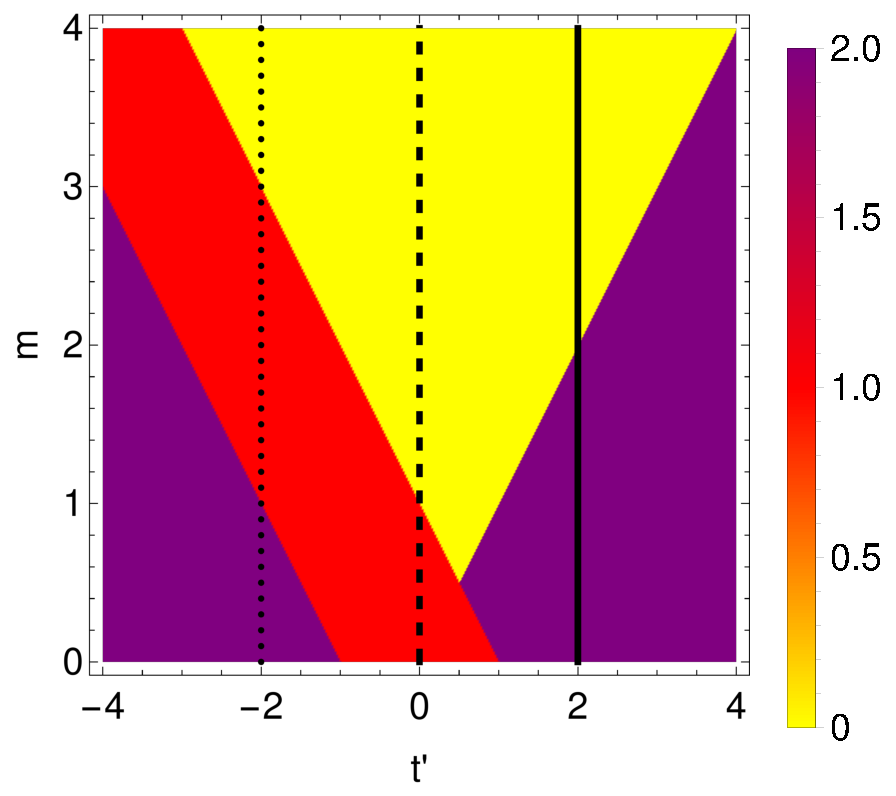
\includegraphics[width=45mm]{phase_diagram2.pdf}
}}\hspace{0mm}

\makebox[0pt]{
\subfloat[$t = 1,t'=-2$, \, $\kappa =\kappa'=0$]{
  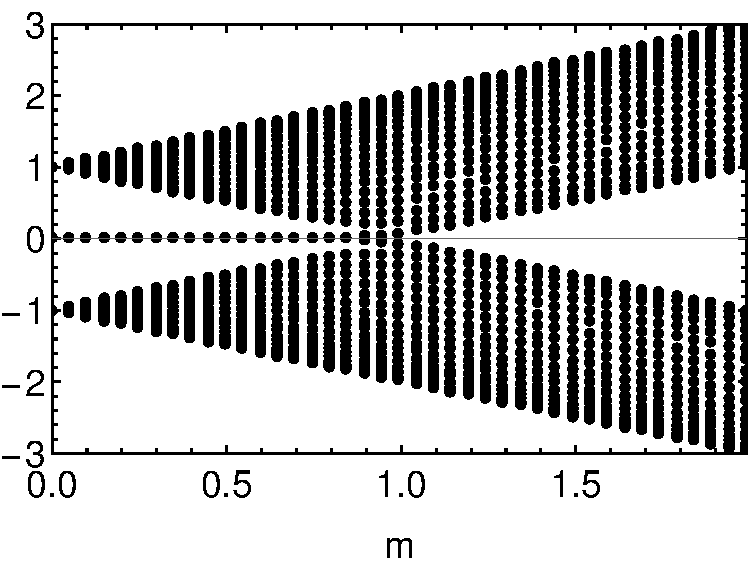
\includegraphics[width=35mm]{1_a.pdf}
}
\subfloat[$t=1,t'=-2$, $\kappa = 0.3, \kappa'=0$]{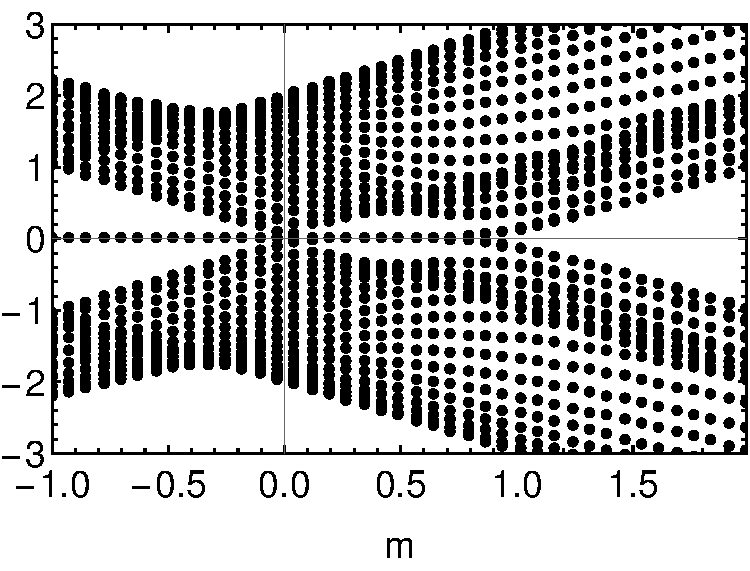
\includegraphics[width=35mm]{1_b.pdf}
}
}\hspace{0mm}

\makebox[0pt]{
\subfloat[$t = 1,t'=-2$, $\kappa = 0,\kappa'=0.3$]{
  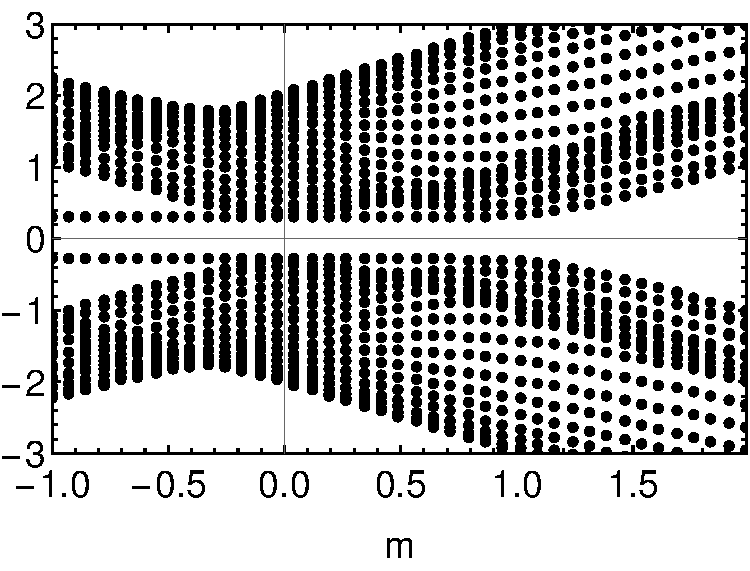
\includegraphics[width=35mm]{1_c.pdf}
}
\subfloat[$t=1,t'=-2$, $\kappa = 0.3,\kappa'=0.3$]{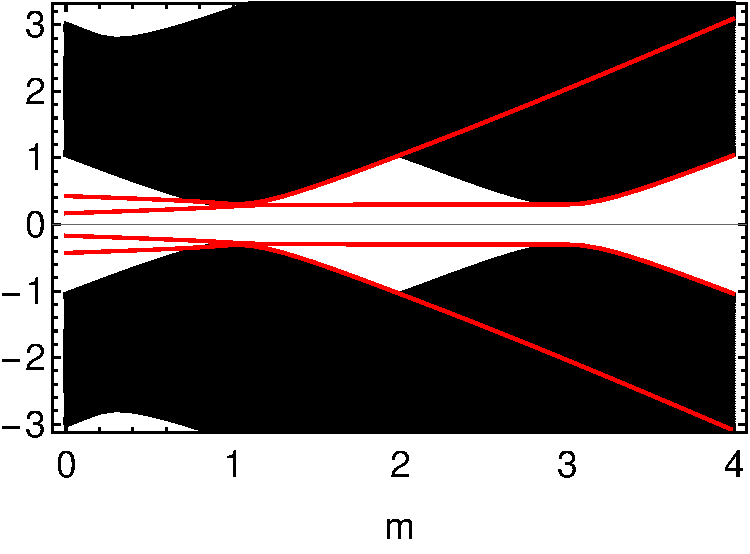
\includegraphics[width=35mm]{1_d.pdf}
}
}
\caption{Phase diagram for the system in the $BDI$ class showing the winding number of each region and surface energy spectrum for a cut going through the three differet regions, for different values of $\kappa,\kappa'$.}
\label{bdi_phase_diagram}
\end{figure}

\section{Zak phase and Entanglement spectrum}
Consider a quadratic Hamiltonian in one dimension
\begin{equation}
\mathcal{H} = \sum_{ij,\alpha\beta} c_{i\alpha}^\dagger H_{ij,\alpha \beta}c_{j\beta}.
\end{equation}
We can obtain the single-particle eigenstates as
\begin{align*}
\sum_{j\beta}H_{ij,\alpha\beta} u^{p\mu}_{j\beta} = E_{p\mu} u_{i\alpha}^{p\mu},
\end{align*}
where $[U]_{j\beta,p\mu} = u^{p\mu}_{j\beta}$ is the unitary matrix that diagonalizes $H$. The polarization can be obtained as the many-body average of the position operator, but it has to be regularized for periodic boundary conditions \cite{Resta1997}. We can define a position operator for PBC as
\begin{equation}
\hat{X}_{\rm PBC} = e^{-i\frac{2\pi}{L}\hat{X}},
\end{equation}
where $\hat{X}$ is the sum of all the single-particle position operators. We can consider then the many-body average of the position operator over the ground state, defined as
\begin{align*}
\expval{\hat{X}_{\rm PBC}}_0 \equiv -\frac{L}{2\pi} \rm{ Im\, Ln }\bra{\Psi_0}\hat{X}_{\rm PBC}\ket{\Psi_0},
\end{align*}
\carlos{This is the notation used in the Resta paper, but I'm not sure if it's confusing.}

where $\ket{\Psi_0}$ is the many-body ground state. Using that the ground state is a Slater determinant of the single-particle eigenstates, $\ket{u^{p\mu}}$, it can be rewritten as
\begin{align*}
\expval{\hat{X}_{\rm PBC}}_0 = -\frac{L}{2\pi} \rm{Im \, Ln}\, {\rm det} \, \tilde{S},
\end{align*}
where the matrix $\tilde{S}$ is obtained from another matrix S with elements
\begin{equation}
S_{p\mu,q\nu} = \sum_{j\alpha}u^{p\mu\, \ast}_{j \alpha} e^{-i\frac{2\pi}{L}j}u^{q\nu}_{j \alpha}
\end{equation}
by restricting it to the space of occupied single-particle states. The Zak phase can now be obtained as
\begin{equation}
\gamma = \expval{\hat{X}_{\rm PBC}}_0\frac{2\pi}{L} + \frac{1}{2}
\end{equation}
\carlos{There is an extra 1/2 factor compared to Restas's formula which I don't know where it is coming from.}
The correlation function in position space is given by
\begin{align*}
C_{ij}^{\alpha \beta} = \expval{c_{i\alpha}^\dagger c_{j\beta}}.
\end{align*}
In terms of the fermions that diagonalize the Hamiltonian, 
\begin{align*}
& \gamma_{i\alpha} = \sum_{j\beta}u_{j\beta}^{i\alpha \, \ast} c_{j\beta} \\
& c_{i\alpha} = \sum_{j\beta} u^{j\beta}_{i\alpha} \gamma_{j\beta}
\end{align*}
we have
\begin{align*}
C_{ij}^{\alpha \beta} =& \sum_{pq,\mu\nu} u^{q\nu }_{j\beta} u^{p\mu \, \ast}_{i\alpha} \expval{\gamma^\dagger_{p\mu} \gamma_{q\nu} } \\
=&  \sum_{p\mu} u^{p\mu }_{j\beta} u^{p\mu \, \ast}_{i\alpha} \expval{\gamma^\dagger_{p\mu} \gamma_{p\mu} } \\
=&  \sum_{p\mu} u^{p\mu }_{j\beta} u^{p\mu \, \ast}_{i\alpha} [1-{\rm sign}(E_{p\mu})]/2.
\end{align*}
The first term is simply a kronecker delta between both sets of indeces. The second term can be rewritten as
\begin{align*}
UD(\abs{D})^{-1}U^\dagger =& UD(D^2)^{-1/2}U^\dagger \\
=& U D U^\dagger (U D^2 U^\dagger)^{-1/2} \\
=& H(H^2)^{-1/2},
\end{align*}
where $D$ is the diagonal Hamiltonian, $H=UDU^\dagger$. Finally the correlation function can be obtained in position space as
\begin{align*}
C_{ij}^{\alpha \beta} =& \frac{1}{2}\left[I - H/ (H^2)^{-1/2} \right]_{ij, \alpha \beta}
\end{align*}
The single-particle entanglement spectrum (ES) is then obtained as the spectrum of the subsystem correlation function obtained after bisecting the system into two equal parts. 

In the ES we can differentiate between two types of eigenvalues, which we denote by $\xi$. The ones at $\xi_b = 0,1$ correspond to bulk states while for the ones in between, $0<\xi_{l,r}<1$, we find their correspondent eigenstate localized in either the left, $\xi_l$, or right, $\xi_r$, virtual edge \cite{Peschel2008}. 
\mariac{introduce entanglement energy, relation between C and energies}
\section{Homogeneous system}

\subsubsection{Nearest-neighbor hopping}


For symmetry-protected topological systems in one dimension there is a well-known relation between ES and the Zak phase \cite{Peschel2008}. The Zak phase, which is quantized, is zero whenever there is an even number per edge of eigenvalues at $\xi = 1/2$, and $\pi$ when the number is odd. Beyond symmetry protected systems, there was observed that in the fully dimerized SSH chain, with only a single mode present in the ES, the Zak phase is equal to the midgap eigenvalue \cite{Ryu2006}. For cases with more edge modes present in the ES it has been shown that the Zak phase follows the midgap eigenvalues qualitatively \cite{Huang2012,Huang2012-2}. The first result we show is that in systems with nearest-neighbor hopping, like the SSH chain, one can obtain the Zak phase by ordering the eigenvalues of the ES, $\xi_1 < \xi_2 < ...$, and computing
\begin{equation}
\chi = \frac{1}{2}\left(\sum_j (-1)^j \xi_j+N_A\right) \, {\rm mod} \, 1,
\label{eqplusminus}
\end{equation}
where $N_A$ is the number of electrons in the ground state in region A, which in the thermodynamic limit fulfills
\begin{equation}
\lim_{L \rightarrow \infty} \gamma = \lim_{L \rightarrow \infty} \chi.
\end{equation}

In the case where there is only one finite eigenvalue in  the ES, like in the fully dimerized limit of the SSH chain, we recover the equality between the midgap eigenvalue and the Zak phase. In Fig.\ref{huang} we show show the dashed cut in the phase diagram shown above, which is equivalent to an SSH chain. We see that even though the ES has finite eigenvalues in the trivial phase these are double-degenerate so that they cancel each other. In the case where we break the symmetry we see that there is one main midgap eigenvalue, so that the Zak phase follows it very closely, but as the midgap eigenvalue approaches the bulk, the contribution from the other modes becomes more relevant and the Zak phase start to deviate from the midgap eigenvalue.
\begin{figure}[h!]
\centering
\makebox[0pt]{
\subfloat[$t = 1,t'=0$, \, \,$\kappa =\kappa'=0$]{
  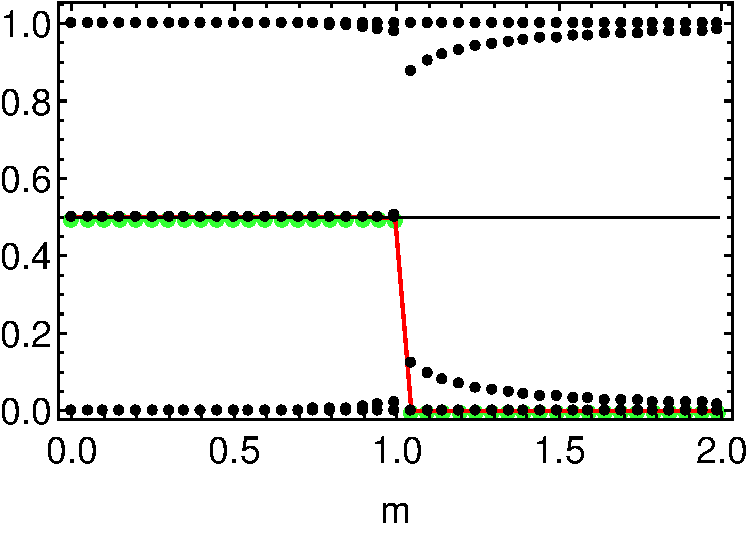
\includegraphics[width=35mm]{2_a.pdf}
}
\subfloat[$t=1,t'=0$, $\kappa = 0.3, \kappa'=0$]{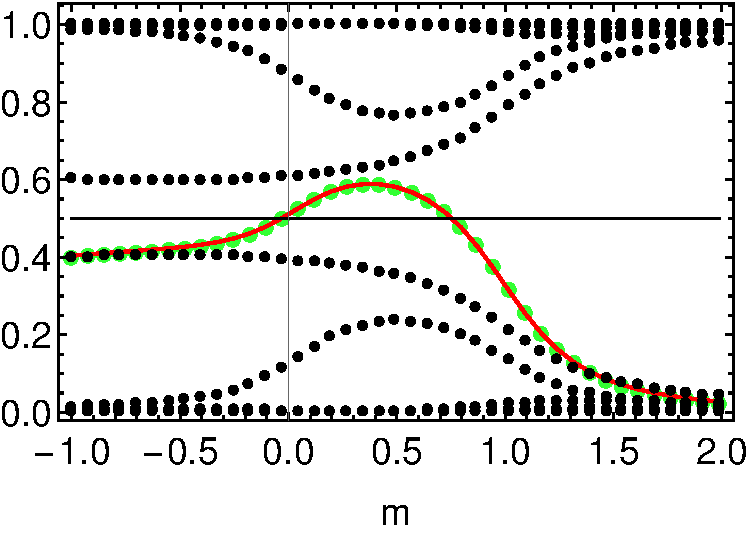
\includegraphics[width=35mm]{2_b.pdf}
}
}
\caption{Entanglement spectrum (black), $\chi$ (green) and $\gamma$ (red) for a cut in the phase diagram through the $\nu = 1 \rightarrow \nu = 0$ transition (dashed line in the phase diagram) for $t'=0$ and different values of $\kappa$.}
\label{huang}
\end{figure}

\subsubsection{General case}

In expression 	\eqref{eqplusminus} we assigned a charge of $\pm1/2$ to each entanglement eigenstate depending on the eigenvalue ordering. 
In order to generalize this to systems with longer-range hopping one needs to know how to properly assign this $\pm 1/2$ charge to each entanglement mode. We found that this is done according to their localization, so we have
\begin{equation}
\chi = \frac{1}{2} \left( \sum_{i\in r}\xi_i-\sum_{i\in l}\xi_i \pm \sum_{i\in b}\xi_i  + N_A \right) \quad {\rm mod} \quad 1,
\label{loceq}
\end{equation}
by defining $ \chi$ modulo $1$ we make the charge of the bulk modes irrelevant but in the next section we will have to take a closer look at it. We find the charge of the edge modes by computing $\expval{\hat{X}}_i$ and seeing if it is above or below $L/4$. In the case the ES is double degenerate at most, left and right edge states might mix but one will always classify one state of the pair as left and the other one as right, this is however not the case when the degeneracies are higher than two-fold. In order to ensure that we obtain edge modes localized at one edge, instead of $C_A$ we diagonalize $C_A + \lambda C_A\hat{X}C_A$ (\carlos{Explain why it does not work in general}), where $\hat{X}$ is the position operator and $\lambda$ is a small parameter that vanishes in the thermodynamic limit. 

The reason expression~\eqref{loceq} simplifies so much for systems with only nearest-neighbor hopping is that it is known that in this case the eigenstates of $C_A$ always come with an alternating edge localization (left-right-left...), so that the signs assigned are always $ \pm(+-+-+-...)$. Their eigenvalues are also related, so that the modes can only cross each other if all of them do so two by two, so that it just ammounts to a global minus sign.

This relation between the Zak phase and the entanglement spectrum is a consequence of an identity between the Zak phase and the many-body entanglement spectrum previously found for infinite chains \cite{Zaletel2014}. In Appendix A we modified this derivation to account for the periodic boundary conditions we use and show how their result reduces to Eq.~\eqref{loceq} when expressing it in terms of the ES.

In Fig.\ref{2} we show an example that highlights the importance of the localization structure of the ES. For the solid line cut in the phase-diagram, with the $\nu = 2 \rightarrow 0 $ transition, two ES that seem at first very similar result in very different Zak phases. This happens because of how the two symmetry breaking terms split the four-fold degenerate midgap states. While $\kappa'$ splits them into two two-fold degenerate pairs whose contribution cancels, $\kappa$ split thems into two $left-left$ and $right-right$ pairs, with a finite contribution to the Zak phase. We also show the cut through the dotted line that shows all possible phases to illustrate how our results also apply to more complex ES. 

\begin{figure}[h!]
\centering
\makebox[0pt]{
\subfloat[$t = 1, t' = 2,$   $\kappa =0.3, \kappa' = 0$]{
  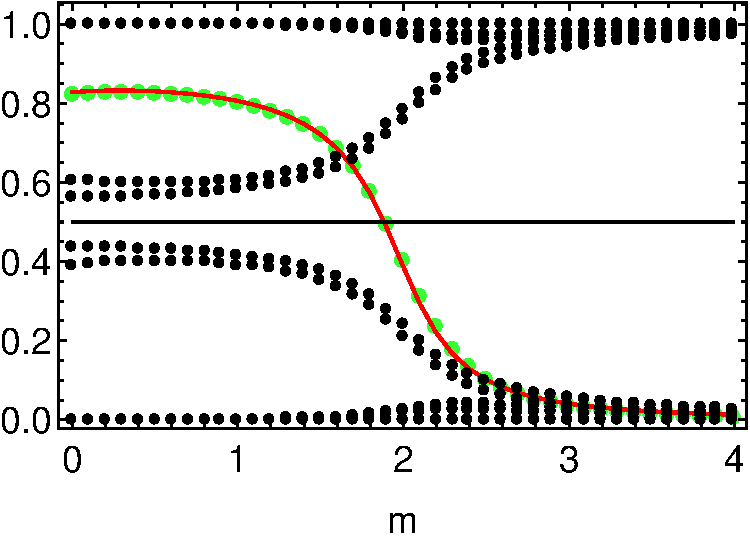
\includegraphics[width=35mm]{3_a.pdf}
}
\subfloat[$t = 1, t' = 2,$ $\kappa = 0, \kappa' = 0.3$]{
  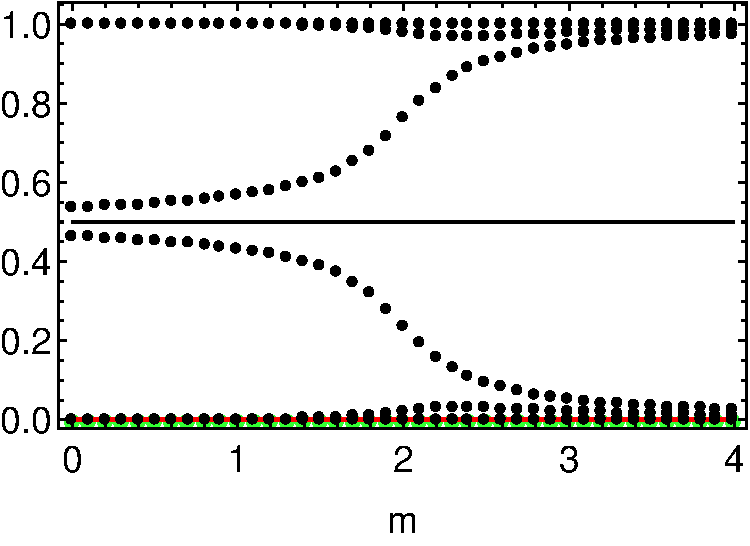
\includegraphics[width=35mm]{3_b.pdf}
}
}\hspace{0mm}

\makebox[0pt]{
\subfloat[$t = 1, t' = -2,$ $\kappa = 0.3, \kappa' = 0$]{
  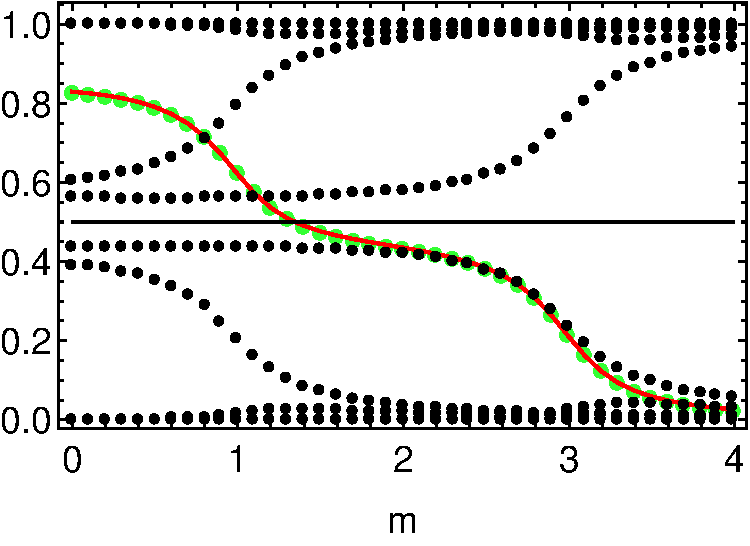
\includegraphics[width=35mm]{3_c.pdf}
}
\subfloat[$t = 1, t' = -2,$ $\kappa = 0, \kappa' = 0.3$]{
  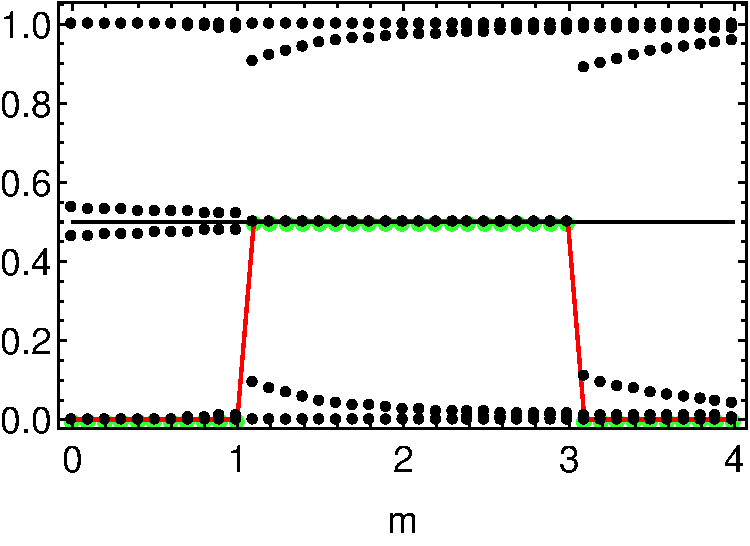
\includegraphics[width=35mm]{3_d.pdf}
}
}
\caption{Entanglement spectrum (black), $\chi$ (green) and $\gamma$ (red) for two different cuts,  continuous line for a,b, and dotted line for c,d plots, Showing a more diverse ES where more than one midgap state is present. }
\label{2}
\end{figure}

Using the fact that $N_A = \Tr C_A$ we can rewrite $\chi$ as
\begin{equation}
\chi = \left(\sum_{i\ in r} \xi_i+ \sum_{i\in b}\xi_i\right) \, {\rm mod} \, 1.
\end{equation}
A simpler way one can compute this quantity is by obtaining $C_A$ for an open chain, labeled as $C_A^{ o}$. For a long enough chain the right eigenvalues will remain the same, as we still place a virtual cut in the middle of the chain but the left eigenvalues will no longer be present, so that one can simply compute
\begin{equation}
\chi = \Tr C_A^{o} \, {\rm mod} \, 1.
\end{equation}
This method however will introduce a stronger finite size effect and as we will discuss below it only works for homogeneous systems. \carlos{I don't know if its worth it to introduce in this paper. Then I dont know what to do for the ES = winding. }



\section{Inhomogeneous systems}


In reference \cite{Zaletel2014} translational invariance was used to derive the relation between the many-body entanglement spectrum and the Zak phase. If this symmetry is broken by, for example, adding weak disorder to the system, this will modify slightly the eigenvalues of the reduced density matrix but not the charge assignment in Eq.~\eqref{zaletel} in the Appendix. The left side of Eq.~\eqref{zaletel} will be cut independent while the right side is not, and therefore cannot be correct. 

We are interested therefore in finding a cut-independent quantity from the ES that might still result in the Zak phase. The first thing one can do is to do an average over the different cuts. Naively one would cut-average the expression in Eq.~\eqref{loceq}, however the average of a circular quantity is not well defined. We defined $\chi$ modulo 1 because the Zak phase is also defined modulo 1, but it also served the purpose of getting rid of the sign choice for the bulk modes, which is problematic. As we do for the edge state, we can choose a sign for the bulk modes in the following way
\begin{equation}
g_i=
\begin{cases}
 +1 &,\rm{if} \expval{\hat{X}}_i > L/4  \\
 -1 &,\rm{if} \expval{\hat{X}}_i < L/4.
\end{cases}
\end{equation}
So that now we define
\begin{equation}
\chi_s = \frac{1}{2} \left( \sum_{i\in r}\xi^s_i-\sum_{i\in l}\xi^s_i + \sum_{i\in b}g_i^s \xi^s_i  + N_A \right),
\end{equation}
obtained for cuts at $s$ and $s+L/2$ and the cut-average is given by
\begin{equation}
\bar{\chi} = \frac{1}{L}\sum_{s=1}^L \chi_s.
\label{batcutavg}
\end{equation}
By adding the perturbation proportional to $C_A\hat{X} C_A$ the bulk modes also localize. As we move through the different cuts the average position of the bulk modes moves slightly. For most modes this will not affect the assigned sign, but for the modes near the middle of subsystem $A$ it might be that for strong enough inhomogeneity that the mode crosses $L/4$ and the sign changes. We find that in order for us to get the correct result the contribution from the bulk modes should be constant across cuts, so we have to find a way of correcting for these jumps of $1$ in $\chi_s$. 

\subsubsection{Continuous inhomogeneity}

In the case we have a continuous inhomogeneity one can obtain a new quantity $\chi'_s$ with a constant bulk contribution, by assuming that the discontinuities of $\chi_s$ above some threshold, $h$, are due to these unphisical changes of sign for the bulk states and eliminating them by shifting it by an integer number so that
\begin{equation}
\chi_{s+1}'-\chi'_s < h
\end{equation}
and it is continuous. $\chi'_s$ can now be cut-averaged to obtain the Zak phase. In figure \ref{inh} we show this for a continuous profile for $\kappa_s$. We see that $\chi_s$ in fact presents jumps of $1$ but once we correct them in $\chi'_s$, its cut average results in the Zak phase. We also see the same for a disordered $\kappa_s$. Even though the disorder is relatively strong we see that $\chi_s'$, after the artificial jumps are eliminated, is fairly continuous, which allows us to use this method even for strong inhomogeneity, as long as we can identify this jumps. 



\begin{figure}[h!]


\centering
\makebox[0pt]{
\subfloat[]{
  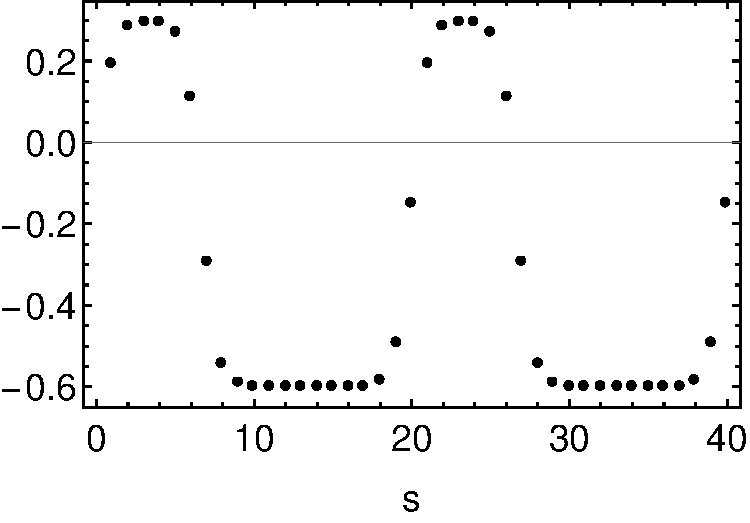
\includegraphics[width=40mm]{4_a.pdf}
  \label{inha}
}
\subfloat[ ]{
  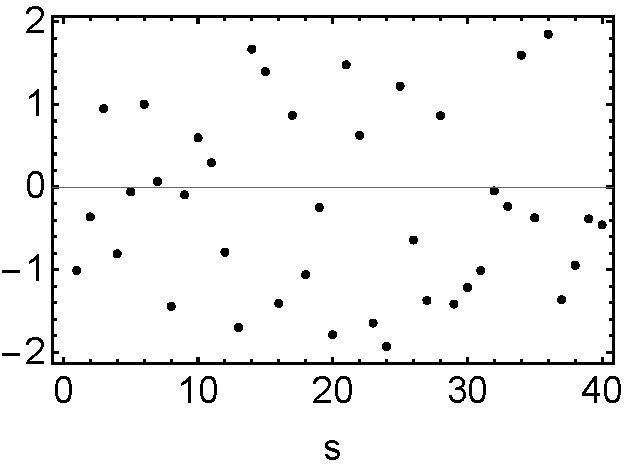
\includegraphics[width=40mm]{4_b.pdf}
}
}\hspace{0mm}

\makebox[0pt]{
\subfloat[]{
  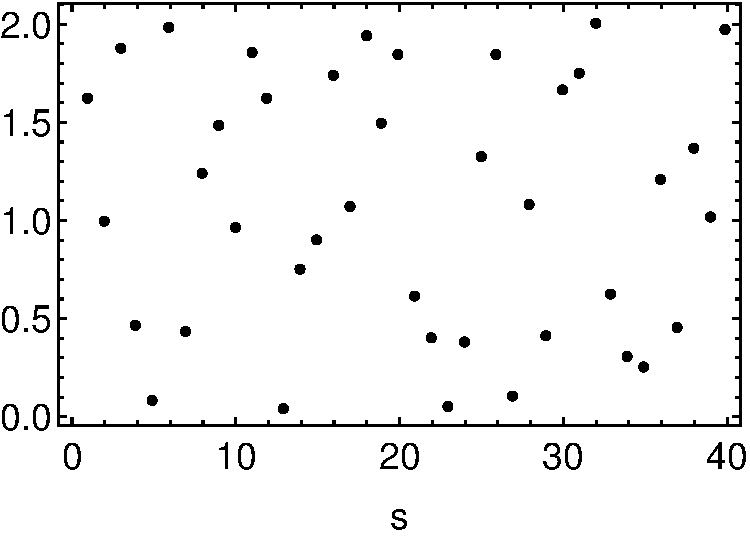
\includegraphics[width=40mm]{4_c.pdf}
}
\subfloat[]{
  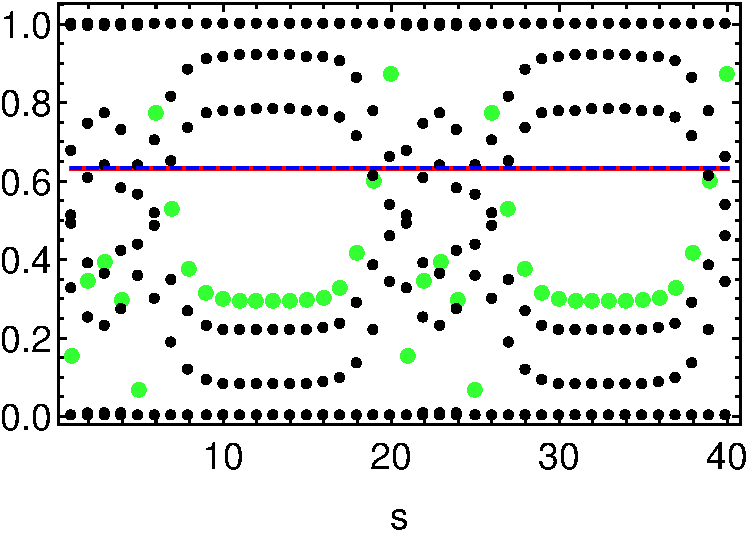
\includegraphics[width=40mm]{4_d.pdf}
}
}\hspace{0mm}

\makebox[0pt]{
\subfloat[]{
  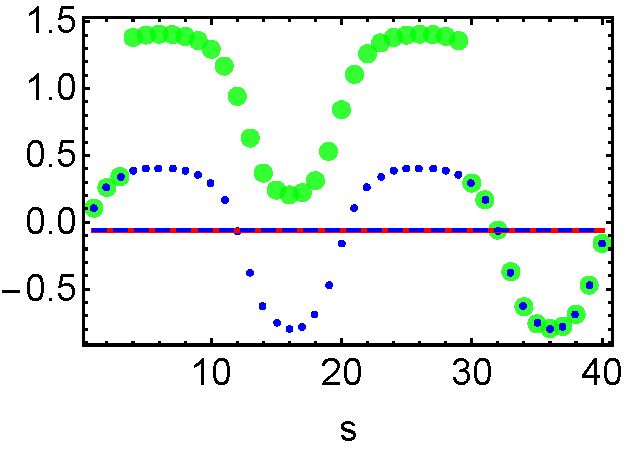
\includegraphics[width=40mm]{4_e.pdf}
}
\subfloat[]{
  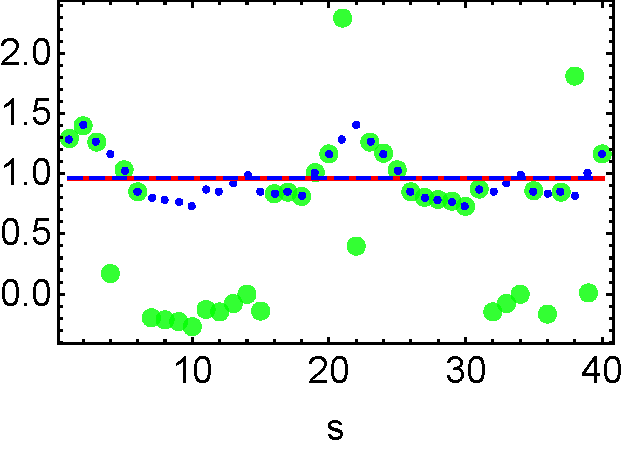
\includegraphics[width=40mm]{4_f.pdf}
}
}

\caption{Using the parameters \label{inh}$t=1,t'=2,m =1$, we show our results for two different profiles for $\kappa_s$, one continuous (a) and one with disorder (b). In (c) and (d) we show the ES (black) and $ \chi_s \, {\rm mod} \, 1$ (green). In (e) and (f) we show $\chi_s$ (green), $\chi'_s$ (blue dots), $\gamma$ (red) and $\expval{\chi'_s}_{\rm cuts}$ (blue dashed) }

\end{figure}

In some cases, this calculation simplifies a bit more. Note that, in the case where one can tell a priori that the width of $\chi'_s$ is lower than 1, as in the example with disorder, to recover $\chi_s'$ one can simply take the modulo 1 and adding an offset, so for instance in the example with disorder we can obtain
\begin{equation}
\chi'_s = ([\chi_s-1/2] \, {\rm mod} \, 1)+1/2.
\end{equation}
One can then cut-average the resulting $\chi_s \, \rm{mod} \,1$ in the same way to obtain the Zak phase. This cannot be done in the first example because as we already see in Fig.\ref{inh}.c, $\chi_s \, \rm{mod} \,1$ wraps aroud the full range, so that there is no offset that will allow us to average it in a well-defined way.


In Fig.\ref{disorder} we show $1-\expval{\chi_s}_{\rm cuts}/\gamma$ for different system lengths for system with weak disorder, as well as the disorder average of $1-\chi_0/\gamma$. For both cases the error seems to vanish in the thermodynamic limit. For small systems both errors are very similar, which suggests that it comes strictly from a systematic finite size error in the computation of either the Zak phase or the ES which is system-independent. For larger systems the disoder average is more dispersed, probably due to the number of configurations considered not being high enough. 

\begin{figure}[h]
\centering
\makebox[0pt]{
\subfloat[$t = 1, t' = 2, m=1, \kappa_s \in (-1,1)$]{
  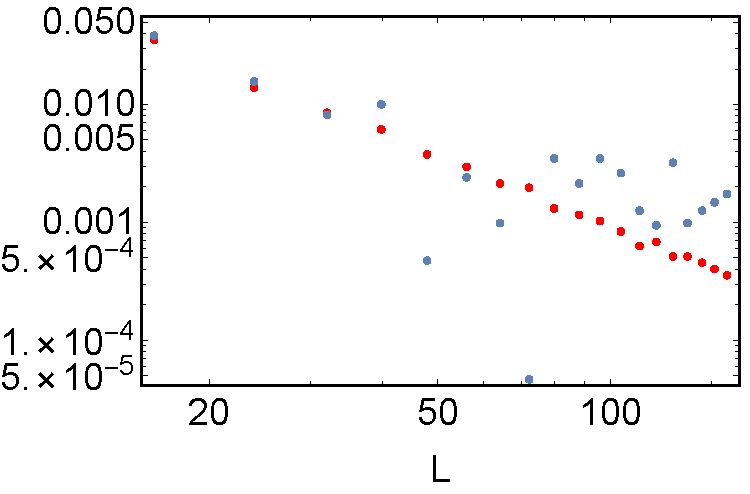
\includegraphics[width=65mm]{disvscut.pdf}
}
}
\caption{We show $1-\expval{\chi_s'}_{\rm cuts}/\gamma$ (red) and $1-\expval{\chi_s'}_{\rm dis}/\expval{\gamma}_{\rm dis}$. The cut average seems to do as good or better than the disorder average. For small systems it seems that both errors are similar, pointing to a systematic finite size error in the computation of either the Zak phase or the ES. For larger systems the error in the disorder average is more spread, which suggests that one should average more configurations.}
\label{disorder}
\end{figure}

\subsubsection{Wannier states, L/4 crossing fix}


\begin{figure}[t]
\centering
\makebox[0pt]{
\subfloat[$\expval{\hat{X}}_{i,s}$ for different cuts, for the entanglement eigenstates such that $\xi_i < 1/2$ (black) and the Wannier states (red)]{
  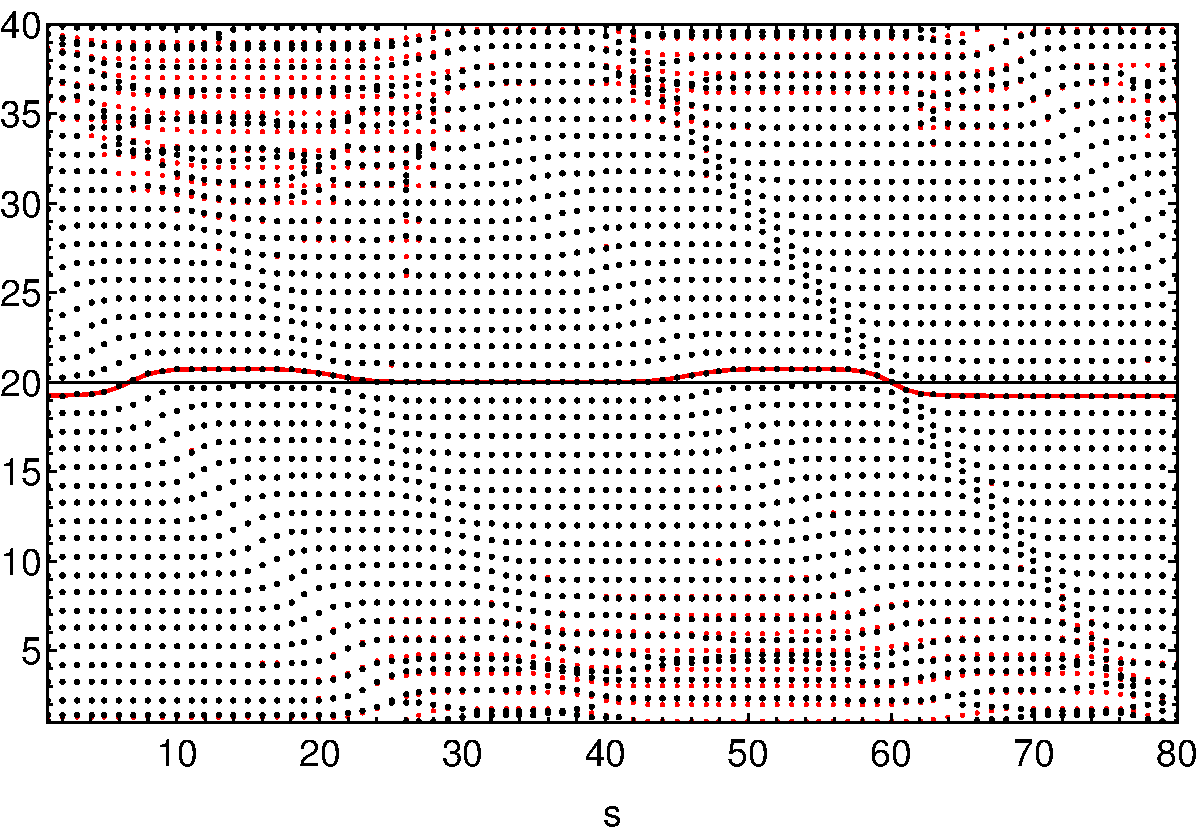
\includegraphics[width=90mm]{loca.pdf}
}}\hspace{0mm}

\makebox[0pt]{
\subfloat[$\chi_s$]{
  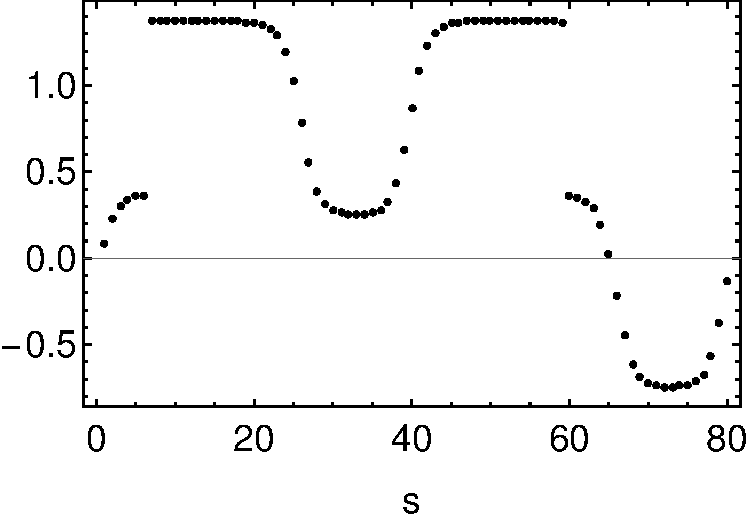
\includegraphics[width=45mm]{wan1.pdf}
}
\subfloat[$\chi_s'$ ]{
  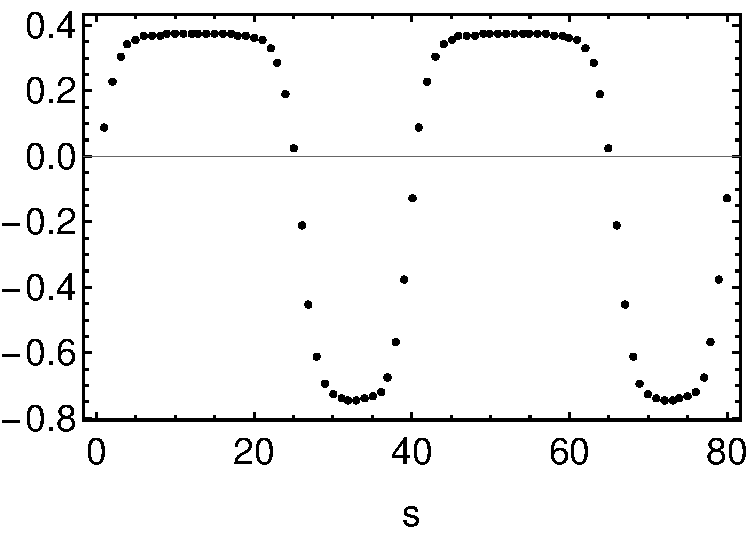
\includegraphics[width=45mm]{wan2.pdf}
}
}

\caption{For the same parameters as used in Fig.5.a,c,e we show the expectation value of the position for the ES eigenstates (black) and the Wannier states (red), showing that the latter are a good approximation of the former in the bulk. We highlight by a continuous red line the bulk mode that crosses $L/4$ which causes the jumps in $\chi_s$. In (b) we show again $\chi_s$ (black) and the correction for the sign switch (red). In (c) $\chi_s'$ is reconstructed via this method, showing the same result as we had before.}
\label{wan}
\end{figure}


In a general case where the discontinuities are too strong and we do not know how to correct for these jumps as explained before one has to take a closer look into the bulk states to ensure a consistent sign assignment. As we mentioned above the bulk states farthest away from the edges are the problematic ones. They are also the ones best approximated by the Wannier states obtained from the chain with periodic boundary conditions, as the eigenstates of 
\begin{equation}
C\hat{X}_{\rm PBC}C
\end{equation}
where $\hat{X}_{\rm PBC} = \exp\{i 2\pi \hat{X}/L\}$. Similar to when we go through different cuts labeled by $s$, we now consider the Wannier states dependent on where we define our lattice site 1, shifted by $s$. The obtained Wannier states for $s$ and $s+1$ will be therefore exactly the same, but shifted one lattice site. By considering their average position $\expval{\hat{X}_{PBC}}_{i,s}$ we can define a set of $2L$ Wannier states that depend continuously on $s$, provided that the Hamiltonian is continuous. These Wannier states are then a good approximation for the Bulk states of $C_A$ we find for the different cuts. 
Consider now the quantity $\sum_i\expval{\hat{X}}_{i,s}$. So far everything was $s$ independent as our system was periodic, but by considering the operator $\hat{X}$ we introduce an unphysical boundary so that it will depend on how the lattice sites are defined. If the states do not cross this unphysical boundary then $\sum_i\expval{\hat{X}}_{i,s} = \sum_i\expval{\hat{X}_{\rm PBC}}_{i,s} $ and it will be a constant with $s$. However, when a Wannier state crosses the boundary we obtain the same constant plus $L$. If we put this boundary at $L/4$ the quantity 
\begin{equation}
\delta_s = \frac{1}{L}\left(\sum_i\expval{\hat{X}}_{i,s}-\sum_i\expval{\hat{X}}_{i,0}\right)
\end{equation}
will be 1 (0) when a states has crossed the boundary or 0 (-1) when it has not, depending on the number of states in A at $s=0$, which we take as reference. Depending which state we take as reference will introduce a global integer shift for all cuts, so it is not relevant as it will go away after we average and take the modulo 1. By adding this term to our cut-average we will compensate for when our bulk state in the middle of A crosses $L/4$ and its charge changes, leading to a continuous $\chi_s'$ which can be averaged,
\begin{equation}
\chi_s' = \chi_s + \delta_s
\end{equation} 

In Fig.\ref{wan} we show how this works for the same continuous example as in \ref{inh}. In Fig.\ref{wan}.a we show the expectation value of the position operator for both the entanglement eigenstates (in black) and the Wannier states (in red) for different values of $s$. In Fig.\ref{wan}.b and c we show $\chi_s$, which displays jumps due to a bulk state crossing $L/4$, and $\delta_s$, showing that it properly corrects the sign switch.

This method conceptually works perfectly whenever the bulk states of the ES are equal to the Wannier states, i.e. in the thermodynamic limit, but it is not clear what the small parameter is. It depends on the $\lambda$ used (it should be small enough to not affect ES but large enough to localize the ES eigenstates) but also on the system. Systems with many ES edge modes close to the bulk tend to have a higher finite size effect.

We also find that whenever there is an interphase in our system, and therefore a zero mode in the energy spectrum, the Wannier states are not necesseraly a good approximation of the bulk of finite systems. However, in the cases where we have an interphase but $\chi_s$ is fairly continuous, so that we can correct these jumps, cut-averaging results again in the Zak phase. 

As the sign assigned to the bulk modes becomes relevant in the inhomogeneous case one might think that it is better to use the open chain, $\chi_s = \Tr C_A^{o,s}$, as one avoids the issue of having to assign any signs at all. Although this is true we find another problem. By adiabatically tuning down the coupling between the $L$ and $1$ sites we see that the eigenvalues of the $left$ modes flow to either $0$ or $1$. In the case where this eigenvalues oscillate around $1/2$ for different cuts this leads to discontinuities in the number of bulk modes at $\xi=1$ which again result in an incorrect cut-average and we found no practical way of compensating for these discontinuitiesyfgh. 

\section{Superconducting systems}

The proof in Ref.\cite{Zaletel2014} also breaks down for superconducting systems. However, as we did for systems without translational invariance, one can extend this identity for systems with pairing terms as well. Since one computes the Zak phase from the single-particle Bogoliubov-de Gennes Hamiltonian, we can obtain the correspondent ES and everything discussed above should apply as well. Take for example the kitaev chain, with the following Hamiltonian
\begin{align*}
H =& -\mu \sum_{i} c_i^\dagger c_i - t \sum_{i}\left( c_{i+1}^\dagger c_i + {\rm h.c.}\right) \\
&+  \sum_{i}\left( \Delta c_{i} c_{i+1} + {\rm h.c.}\right).
\end{align*}
Using the spinor $\phi_i^\dagger = (c_i^\dagger, c_i)$, we can rewrite the Hamiltonian as
\begin{align*}
&H = \frac{1}{2}\sum_i \phi^\dagger_i H_{BdG,ij} \phi_j,\\
&H_{BdG,ij} = -\mu \tau_z \delta_{ij} - (t \tau_z + i\Delta \tau_y )\delta_{i,j+1}- (t \tau_z - i\Delta \tau_y)\delta_{i,j-1}.
\end{align*}
Note that by taking $t' = \kappa = \kappa = 0$ in the BDI model, Eq. \ref{bdi_model}, we obtain
\begin{align*}
H_{ij} =& m \sigma_x\delta_{ij} + \frac{1}{2} t \left[(\sigma_x + i \sigma_y)\delta_{i,j+1} + (\sigma_x - i \sigma_y) \delta_{i,j-1} \right],
\end{align*}
which is just the Bogoliubov-de Gennes Hamiltonian of the Kitaev chain by rotating $x$ into $z$ and identifying $\mu = -m, t_{\rm Kit} = -t_{BDI}/2, \Delta = -t_{BDI}/2 $. From Fig.\ref{bdi_phase_diagram} we see that the $BDI$ model transitions from $\nu = 1$ to the trivial phase at $t=0, m=\pm t_{BDI}$, or alternatively, when $\mu = \pm 2 t_{Kit}$, which is the known result for the Kitaev chain. Therefore the results already shown for the BDI model studied here are also applicable to the Kitaev chain.  

\section{Conclusion}

It was previously known that the Zak phase was encoded in the many-body entanglement spectrum. Here we have shown how it is encoded in the single-body entanglement spectrum. This relation is simpler than the one involving the MBES and it provides more insight into the ES. We have furthermore shown how this relation generalizes to inhomogeneous and superconducting systems, where it was not previously shown to be present. Our result also provides a new way of computing the Zak phase for inhomogeneous systems where instead of diagonalizing a $2L\times 2L$ matrix one has to diagonalize $L$ matrices of size $L\times L$, which in some cases might be computationally favorable. (\carlos{can we get insight on this?}). 

\bibliography{references}	

	
\appendix

\section{Appendix A}
	
Consider a chain with periodic boundary conditions. A Schmidt decomposition for two bipartite cuts gives the ground state
\begin{equation}
\ket{\psi} = \sum_{p,q} \ket{p,q}_A s_p \ket{p,q}_B s_q,
\end{equation}
where we assume that the size of each subsystem is big enough so that the cuts can be considered independent of each other. We can now take subsystem B and glue its ends together to obtain the ground state of a ring with a single cut. If we include a flux threading inside the ring we obtain
\begin{equation}
\ket{\psi^\phi} = \sum_p s_p \ket{p,p}_B e^{i\phi Q_p},
\end{equation}
The many-body states $\ket{p,p}_B$ can be built by occupying the different ES eigenstates and are therefore characterized by a set of occupying numbers $\{n\}_p$. The many-body entanglement spectrum can also be expressed in terms of the single-particle one \cite{Alexandrinata2011} as
\begin{align}
s_p^2 =& \prod_{i \in {\rm occ}} \xi_i \prod_{i \in {\rm empty}}(1-\xi_i) \\
=& \prod_i (1-\xi_i)\left(\frac{\xi_i}{1-\xi_i} \right)^{n_i}
\end{align}
And the charge can be assigned so that $Q_p = \sum_{\alpha = b,l,r} q_\alpha\sum_{i \in \alpha} n_i$ with the constrain that $q_r,\pm q_b = q_l-1$ \textcolor{red}{Why?}. As the main result of \cite{Zaletel2014} the Zak phase is then found to be
\begin{align}
e^{i\gamma} = e^{2\pi i \sum_p s_p^2 Q_p}  \bra{\psi^0}\ket{\psi^{2\pi}},
\label{zaletel}
\end{align}
where the monodromy is given by
\begin{align}
\bra{\psi^0}\ket{\psi^{2\pi}} =& \sum_p s_p^2 e^{2\pi i Q_p}.
\end{align}
Consider the exponential term
\begin{align*}
e^{2\pi i (q_L N^p_l + (1-q_l)(N^p_r+N^p_b))} =& e^{2\pi i (q_l N^p_l + (1-q_l)(N-N^p_l))} \\
=& e^{4\pi i q_l N^p_l}e^{2 \pi i (N-N^p_l)}e^{-2\pi i q_l N },
\end{align*}
where $N^p_\alpha = \sum_{i \in \alpha} n_i$ and the total number of electrons, $N = \sum_{\alpha = b,l,r} N^p_\alpha$, is independent of $p$. We will consider two natural choices, $q_l = 1,1/2$, for which we have
\begin{align}
\bra{\psi^0}\ket{\psi^{2\pi}} =& 
\begin{cases}
1 & \text{for} \quad q_l = 1 \\
e^{N\pi i} & \text{for} \quad q_l = 1/2,
\end{cases}
\end{align}
where we used that $\sum_p s_p^2 = 1$. The change in the monodromy between both choices is accompanied by a change in the exponential term in Eq.\ref{zaletel}, so that both charge choices are equivalent.

Expressing the contribution of the many-body entanglement spectrum to the Zak phase in terms of the ES, we have
\begin{align*}
\gamma' = 2\pi \sum_{n_i = 0,1} \left(\sum_{i } n_i q_i\right) \left(\prod_m (1- \xi_m)\left(\frac{\xi_m}{1-\xi_m} \right)^{n_m} \right) ,
\end{align*} 
Consider now its derivative with respect to a particular entanglement eigenvalue
\begin{align}
\frac{1}{2\pi}\frac{\partial \gamma'}{\partial \xi_p} =& \sum_{\{n_k\}=0,1}\left(\sum_{i } n_i q_i\right)\frac{n_p - \xi_p}{\xi_p^{1-n_p}(1-\xi_p)^{n_p}}\\
&\times \left(\prod_{m\neq p} (1- \xi_m)\left(\frac{\xi_m}{1-\xi_m} \right)^{n_m} \right)
\end{align}
where
\begin{equation}
 \frac{n_p - \xi_p}{\xi_p^{1-n_p}(1-\xi_p)^{n_p}} = 
  \begin{cases}
    -1, & \text{for } n_p=0 \\
    1, & \text{for } n_p = 1 \\
  \end{cases}	
\end{equation}
Therefore we have
\begin{align*}
\frac{1}{2\pi}\frac{\partial \gamma'}{\partial \xi_p} =& -\sum_{\substack{\{n_{k\neq p}\}=0,1 \\ n_p = 0}}\left(\sum_{i \neq p} n_i q_i\right)\prod_{m\neq p} (1-\xi_m)\left( \frac{\xi_m}{1-\xi_m} \right)^{n_m} \\
&+ \sum_{\substack{\{n_{k\neq p}\}=0,1 \\ n_p = 1}}\left(\sum_{i \neq p} n_i q_i +q_p\right) \prod_{m\neq p} (1-\xi_m)\left( \frac{\xi_m}{1-\xi_m} \right)^{n_m} \\
=&q_p\sum_{\{n_{k\neq p}\}=0,1} \prod_{k\neq p} (1-\xi_k)\left( \frac{\xi_k}{1-\xi_k} \right)^{n_k} \\
\end{align*}
Expand now the sum  for another occupation number $n_{p'} = 0,1$ 
\begin{align*}
\frac{1}{2\pi}\frac{\partial \gamma'}{\partial \xi_p} =& q_p\sum_{\substack{n_{k \neq p \neq p'}=0,1\\ n_{p'}= 0}} (1-\xi_{p'})\prod_{k\neq p,p'} (1-\xi_k)\left( \frac{\xi_k}{1-\xi_k} \right)^{n_k} \\
&+ q_p\sum_{\substack{n_{k \neq p \neq p'}=0,1\\ n_{p'}= 1}} \xi_{p'}\prod_{k\neq p,p'} (1-\xi_k)\left( \frac{\xi_k}{1-\xi_k} \right)^{n_k} \\
 &=q_p\sum_{\substack{n_{k \neq p \neq p'}=0,1}} \prod_{k\neq p,p'} (1-\xi_k)\left( \frac{\xi_k}{1-\xi_k} \right)^{n_k} 
\end{align*}
doing this for the rest of the occupation numbers we obtain 
\begin{equation}
\frac{1}{2\pi}\frac{\partial \gamma'}{\partial \xi_p} = q_p,
\end{equation}
so that 
\begin{align*}
\gamma =& \gamma' - i\log(\bra{\psi^0}\ket{\psi^{2\pi}})\\
=& \sum_{i}q_i \xi_i - i\log(\bra{\psi^0}\ket{\psi^{2\pi}})\\
\end{align*}
and we have recovered equation \ref{mainl}. 

\end{document}